% ---------------------------------------------------------------------
% HEADER
% Formålet med å legge header til et eget dokument er å garantere at
% oppsettet av dokumentene er likt for alle løsningsforslagene.
% I headeren skjer følgende:
% (1) Dokumentet blir startet
% (2) Pakker blir importert
% ---------------------------------------------------------------------
% ---------------------------------------------------------------------
% HEADER
% Formålet med header er å importere de samme pakkene i alle dokumentene.
% ---------------------------------------------------------------------

% Sett opp dokumentet. Her kan 'twoside' brukes for printing
\documentclass[12pt, a4paper]{article}

% Vi trenger utf-8 for å bruke norske bokstaver: Æ, Ø, Å
\usepackage[utf8]{inputenc}

% Vi setter babel til norsk, da får dokumentegenskaper norske titler
\usepackage[norsk]{babel}

% For å kunne bruke grafikk
\usepackage{graphicx}
\newcommand{\figwidth}{0.75}

% Matematikkpakker fra AMS - American Mathematical Society
\usepackage{amsmath, amsthm, amsfonts, amssymb, mathtools}

% For eventuelle linker, e.g. \href{URL}{text}
\usepackage{hyperref}

% For headers og footers med eventuell logo
\usepackage{fancyhdr}

% Sett marginer manuelt
\usepackage[top = 3cm, left = 3cm, right = 3cm, bottom = 3cm]{geometry}

% For enkle lister, nyttig for oppgave a), b), c), ...
\usepackage[sharp]{easylist}

% Dersom flere kolonner er ønskelig i deler av dokumentet
\usepackage{multicol}

% For luft mellom paragrafer
\usepackage{parskip}

% For logikk assosiert med logoer
\usepackage{ifthen}

% For å finne totalt antall sider
\usepackage{lastpage}

% Annet
\usepackage{enumitem}

\usepackage{polynom}% Polynomer
\polyset{style=C, div=:}

\usepackage{systeme}% Likningssystemer

% Kan brukes når noe stryker ut noe, f.eks 1/n * n, her kan man ta \frac{1}{\cancel{n}} * \cancel{n}
\usepackage{cancel}



% ---------------------------------------------------------------------
% DOKUMENTVARIABLER
% ---------------------------------------------------------------------
\newcommand{\fagkode}{R1}
\newcommand{\semesteraar}{våren 2018}
\newcommand{\forfatter}{Anita G.}
\newcommand{\dokumenttittel}{Løsningsforslag -- Eksamen \fagkode, \semesteraar}

\usepackage{siunitx}


% Set til 'true' og oppgi logo dersom du vil bruke en logo
\newboolean{bruklogo}
\setboolean{bruklogo}{false}
\newcommand{\logonavn}{}



% ---------------------------------------------------------------------
% SETUP
% Formålet med å legge setup til et eget dokument å garantere at headers,
% footers, og øverste del av dokumentet er likt for alle
% løsningsforslagene.
% ---------------------------------------------------------------------
% ---------------------------------------------------------------------
% HEADER
% Formålet med setup er at dokumentene ser rimelig like ut.
% ---------------------------------------------------------------------


% ---------------------------------------------------------------------
% Alternativ font. Kommentert ut fordi Computer Modern (default) er pen
%\usepackage{kmath,kerkis}
%\usepackage[T1]{fontenc}
% ---------------------------------------------------------------------


% ---------------------------------------------------------------------
% Sett opp headers og footers
\ifthenelse{\boolean{bruklogo}}{
% Dersom logo skal brukes, sett logoen oppe til høyre med bredde 4 cm
	\rhead{\includegraphics[width=3.5cm]{\logonavn}}
}{
% Dersom logo ikke skal brukes, sett tom header
	\rhead{}
} 
\rfoot{\thepage}
\cfoot{}
\lhead{}
\lfoot{{\scriptsize Forbedringsforslag? Bidra på \url{https://github.com/tommyod/matte_eksamener_VGS}.}}
\renewcommand{\headrulewidth}{0pt}
% ---------------------------------------------------------------------


% ---------------------------------------------------------------------
% To streker under svaret
\def\answer#1{\underline{\underline{#1}}}
% ---------------------------------------------------------------------


% ---------------------------------------------------------------------
% Start selve dokumentet
% ---------------------------------------------------------------------

\begin{document}
\pagestyle{fancy}
{\bfseries \Large \dokumenttittel} \\
{ \footnotesize Laget av \forfatter 
	\hfill Sist oppdatert: \today 
	\hfill Antall sider: \pageref*{LastPage}}
\hrule
\vspace{1em}
\begin{center}
\fbox{\fbox{\parbox{.90\textwidth}{
	Dette dokumentet er open-source;
	alle kan bidra til å gjøre det bedre.
	Dersom du finner skrivefeil, matematiske feil, eller ser at forklaringene kan være bedre: ikke nøl med å sende inn en endring. 
	Du kan finne siste versjon, og bidra, på GitHub, se:
	\url{https://github.com/tommyod/matte_eksamener_VGS}
}}}
\end{center}


% ---------------------------------------------------------------------
% DOKUMENTSTART - Skriv løsningsforslaget nedenfor
% ---------------------------------------------------------------------	
\section*{Del 1 - uten hjelpemidler}
\subsection*{Oppgave 1}
\begin{easylist}[enumerate]
	\ListProperties(Style2*=,Numbers=a,Numbers1=l,FinalMark={)})
	# Vi skal derivere $f(x) = x^4 - x +2$. Vi bruker regelen $f(x) = x^n \Rightarrow f'(x) = nx^{n-1}$. Vi får da at $f'(x) = \answer{4x^3 - 1}$.
	
	# Her ser vi at funksjonen $g(x) = x^3 \cdot \ln (x)$ er sammensatt av to faktorer $u(x) = x^3$ og $v(x) = \ln(x)$. 
	Vi bruker derfor produktregelen $f(x) = uv \Rightarrow f'(x) = u'v + uv'$, og får da at
	\begin{align*}
	g'(x) &= 3x^2 \cdot \ln(x) + x^3 \cdot \frac{1}{x}\\
			&= 3x^2 \cdot \ln(x) + x^2\\
			&= \answer{x^2(3\ln(x)+1)}
	\end{align*}
	
	# Vi skal derivere $h(x) = e^{2x^2 + x}$.
	Her får vi bruk for kjerneregelen, der vi velger kjernen som $u = 2x^2 + x$. 
	Utregningen blir da
	\begin{align*}
	h(x) = e^{u(x)} \Rightarrow h'(x) 
	&= (e^{u(x)})' \cdot u'(x) \\
	&= e^{u(x)} \cdot (4x + 1) \\
	&= \answer{(4x +1)e^{2x^2 + x}}
	\end{align*}
\end{easylist}


\subsection*{Oppgave 2}
\begin{easylist}[enumerate]
	\ListProperties(Style2*=,Numbers=a,Numbers1=l,FinalMark={)})
	# Vi skal se på uttrykket
	\begin{equation*}
		\frac{1}{2x-2} + \frac{2}{x-3} - \frac{x-2}{x^2 - 4x +3}.
	\end{equation*}
	Først faktoriserer vi nevnerne for å finne fellesnevneren. 
	Nevneren i det første leddet faktoriseres som $2x-2 = 2(x-1)$. 
	Nevneren i det andre leddet kan ikke faktoriseres, mens nevneren i det tredje leddet kan vi faktorisere for eksempel ved bruk av abc-formelen.
	 Etter faktoriseringen ser uttrykket ut slik:
	\begin{align*}
			\frac{1}{2(x-1)} + \frac{2}{x-3} - \frac{x-2}{(x-1)(x-3)}
	\end{align*}
	
	Vi ser dermed at fellesnevneren er $2(x-1)(x-3)$. Vi ganger første ledd med $(x-3)$ i både teller og nevner, andre ledd med $2(x-1)$ og tredje ledd med $2$.
	\begin{align*}
		&\frac{1(x-3)}{2(x-1)(x-3)} + \frac{2 \cdot 2(x-1)}{2(x-1)(x-3)} - \frac{2(x-2)}{2(x-1)(x-3)} \\
		& = \frac{x - 3 +4x - 4 - 2x + 4}{2(x-1)(x-3)} \\
		& = \frac{3x-3}{2(x-1)(x-3)}\\
		& = \answer{\frac{3}{2(x-3)}}
	\end{align*}
	
	# Her må vi ta i bruk logaritmesetningene. Disse er: 
	$\ln(ab) = \ln(a) + \ln(b)$, 
	$\ln\left(a / b\right) = \ln(a) - \ln(b)$ og 
	$\ln(a^x) = x \ln(a)$.
	Vi regner ut på følgende måte:
	\begin{align*}
		&2\ln(x y^3) - \frac{1}{2} \ln \left (\frac{x^4}{y^2} \right) \\
		& = 2(\ln(x) + \ln(y^3) - \frac{1}{2}(\ln(x^4) - \ln(y^2)) \\
		& = 2(\ln(x) + 3\ln(y)) - \frac{1}{2}(4\ln(x) - 2\ln(y))\\
		& = 2\ln(x) + 6\ln(y) - 2\ln(x) + \ln(y)\\
		& = \answer{7\ln(y)}
	\end{align*}
	
\end{easylist}

\subsection*{Oppgave 3}

\begin{easylist}[enumerate]
	\ListProperties(Style2*=,Numbers=a,Numbers1=l,FinalMark={)})
	# Vektoren mellom to punkter $A = (x_1, y_1)$ og $B = (x_2, y_2)$ er gitt ved $\vec{AB} = B -A = [x_2 - x_1, y_2 - y_1]$. 
	Vi regner ut svaret som
	\begin{align*}
		\vec{AB} &= [-1-(-2), -3-(-1)] = \answer{[1,-2]} \\
		\vec{BC} &= [3-(-1),-1-(-3)] = \answer{[4,2]}
	\end{align*}
	
	# Generelt står to vektorer vinkelrett på hverandre dersom $\vec{AB} \cdot \vec{BC} = 0$.
	I denne oppgaven har vi
	\begin{equation*}
		\vec{AB} \cdot \vec{BC} = [1,-2] \cdot [4,2] = 1 \cdot 4 + (-2) \cdot 2 = 4 + (-4) = \answer{0},
	\end{equation*} 
	så vi ser at vektorene står vinkelrett på hverandre.
	
	# Vektorene $\vec{CD}$ og $\vec{AB}$ er parallelle dersom $\vec{CD} = k \cdot \vec{AB}$, der $k$ er et tall. 
	Vi finner først $\vec{CD}$ på samme måte som vi fant vektorene i oppgave a). 
	\begin{align*}
		\vec{CD} &= [t-3,t^2 + 2- (-1)] = [t-3,t^2 + 3] \\
		\vec{CD} & = k \cdot \vec{AB}\\
		[t-3,t^2 + 3] & = k \cdot [1,-2]  = [k,-2k]
	\end{align*}
	To vektorer er like dersom både $x$ og $y$ koordinatene er like.
	Vi får altså to likninger med to ukjente: 
	\begin{align*}
		t-3 &= k \\
		 t^2 + 3 &= -2k 
	\end{align*}
	Den første likningen gir oss et uttrykk for $k$.
	Dette setter vi inn i den andre likningen og løser for $t$.
	Vi ser at
	\begin{align*}
			&t^2 + 3  = -2(t-3)\\
			&t^2 + 3  = -2t + 6\\
			&t^2 +2t -3 = 0.
	\end{align*}
	Vi bruker så abc-formelen, og får $t = 1$ eller $t=-3$.
	Med andre ord er $\vec{CD}$ og $\vec{AB}$ parallelle dersom $\answer{t = 1}$ eller  $\answer{t = -3}$.
\end{easylist}

\section*{Oppgave 4}
\begin{easylist}[enumerate]
	\ListProperties(Style2*=,Numbers=a,Numbers1=l,FinalMark={)})
	
	# Dersom $P(x)$ er et polynom, går en divisjon $P(x) : (x-a)$ hvis og bare hvis $P(a) = 0$. 
	Vi må sjekke hvilke verdier av $k$ som oppfyller likningen $f(1)= 0$.
	\begin{align*}
		f(1) = (1)^3 + k \cdot (1) + 12 &= 0 \\
		1+k+12 & =0 \\
		k & =  \answer{-13}
	\end{align*}
	
	# Vi har nå at $f(x) = x^3 - 13x + 12$. 
	Vi vet at $f(x)$ er delelig med $(x-1)$, derfor utfører vi en polynomdivisjon med $(x-1)$ for å faktorisere $f(x)$. 
	Vi vil få et andregradspolynom etter polynomdivisjonen som vi kan faktorisere videre ved hjelp av abc-formelen. 
	\newline
	\polylongdiv{x^3 -13x+12}{x - 1} 
	\newline
	
	Fra abc-formelen ser vi at $(x^2 + x - 12)$ kan faktoriseres til $(x+4)(x-3)$. 
	Vi setter sammen alle de lineære faktorene, og får da at $f(x)$ kan faktoriseres som 
	$f(x) = x^3 - 13x + 12 = \answer{(x-1)(x+4)(x-3)}$.
	
	# Vi skal løse ulikheten
	\begin{equation*}
		\frac{x^2 + x -12}{x-1} \geq 0.
	\end{equation*}
	Fra forrige oppgave vet vi at telleren kan faktoriseres til $(x+4)(x-3)$, som vil si at vi kan skrive brøken som $$\frac{(x+4)(x-3)}{x-1}$$
	
	Vi lager fortegnsskjema som vist nedenfor.
	\begin{figure}[ht!]
		\centering
		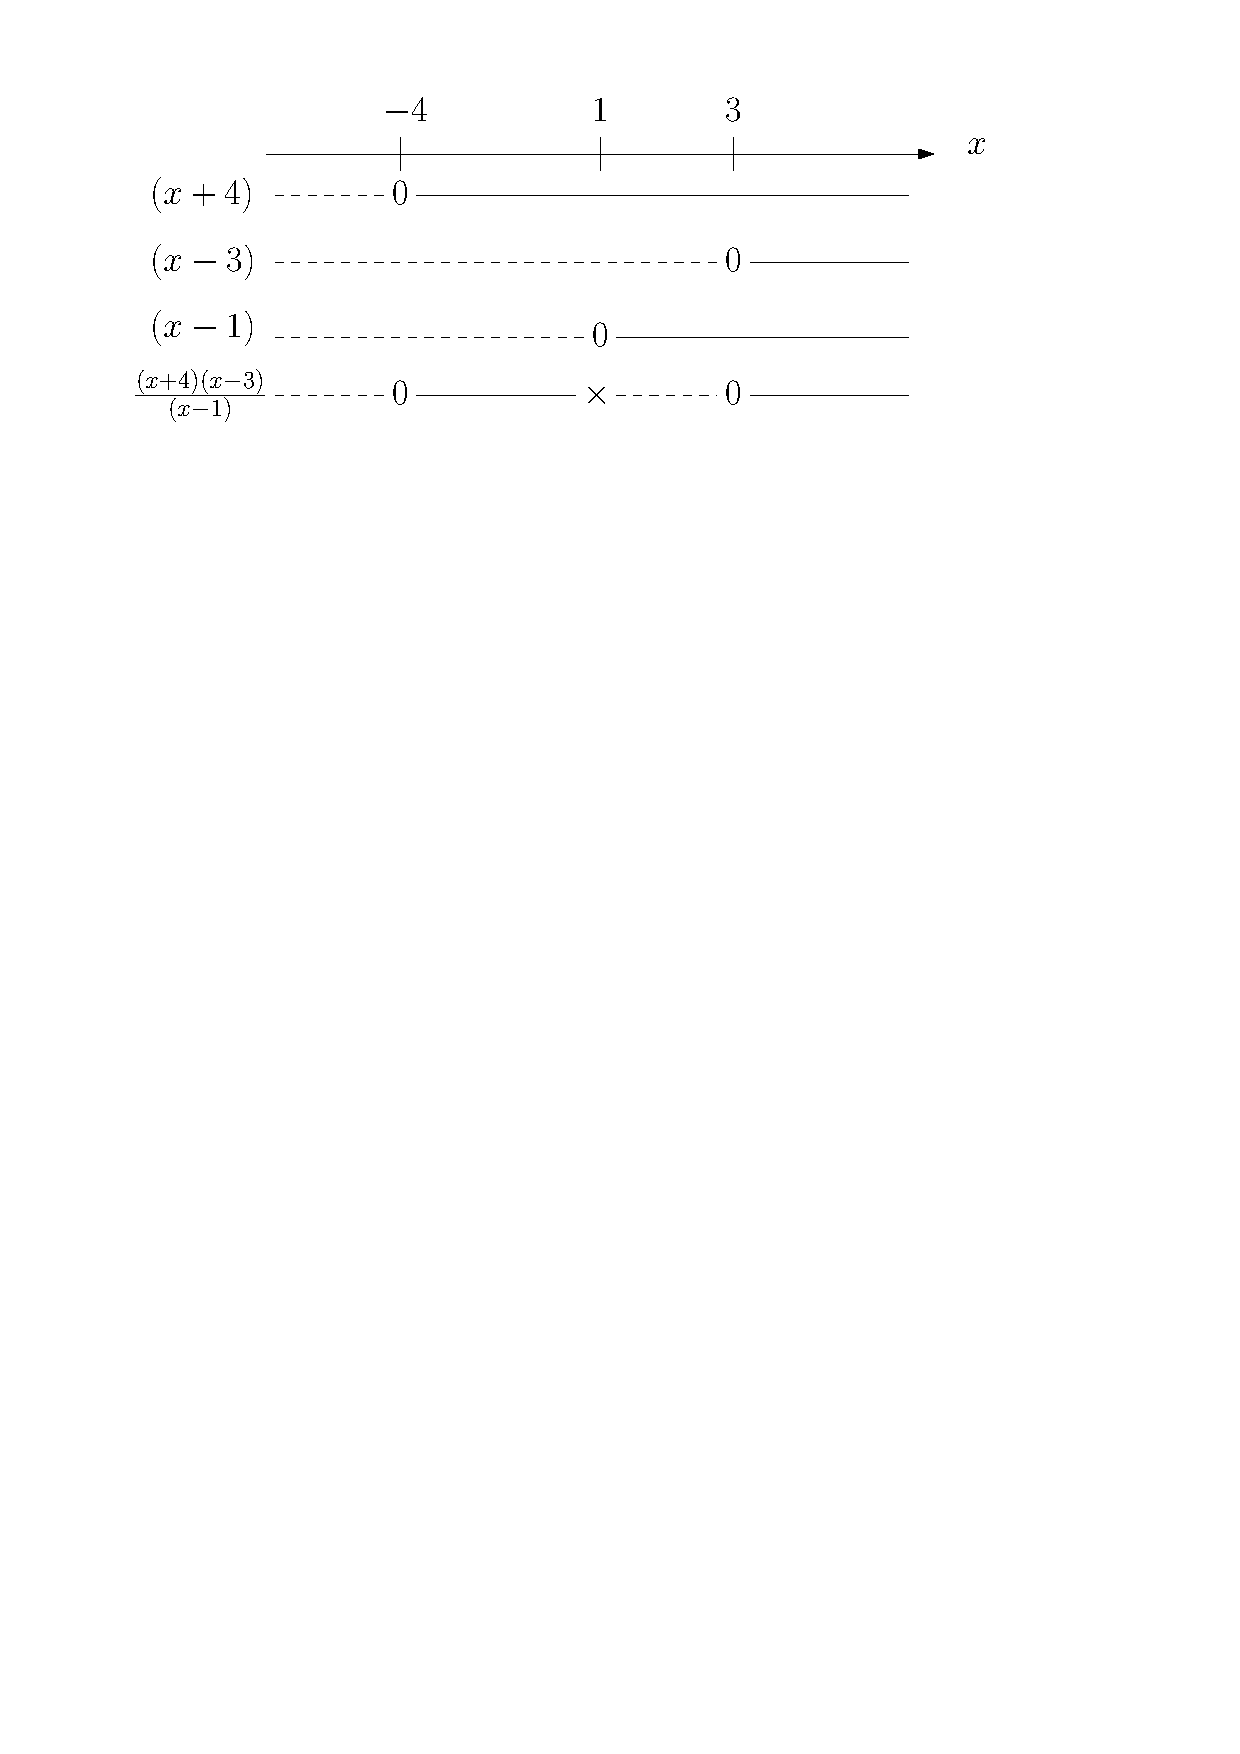
\includegraphics[width=0.725\linewidth]{figs/del1_oppg4c.pdf}
		\label{fig:del1_oppg4c}
	\end{figure}
	
	Fra fortegnsskjemaet ser vi at ulikheten
	\begin{equation*}
		\frac{(x+4)(x-3)}{x-1} \geq 0
	\end{equation*}
	når \answer{$-4 \leq x < 1$ og når $x \geq 3$}.
	
\end{easylist}

\subsection*{Oppgave 5}

\begin{easylist}[enumerate]
	\ListProperties(Style2*=,Numbers=a,Numbers1=l,FinalMark={)})
	
	
	#  Vi skal finne sannsynligheten for at laderen kommer fra leverandør A \emph{og} at den er defekt. 
	Hendelsen at laderen kommer fra leverandør A kaller vi for $A$.
	Vi skal her finne sannsynligheten $P(A \mid \textnormal{defekt})$, og bruker produktsetningen til å regne ut
	\begin{align*}
			P(A \: \cap \: \textnormal{defekt}) & = P(A) \cdot P(\textnormal{defekt}  \mid A) \\
			& = 0.4 \cdot 0.03 \\
			& = 0.012
	\end{align*}
	\answer{Sannsynligheten for at laderen er fra leverandør A og er defekt er 1.2 \%.}
	
	# For å bestemme sannsynligheten for at en lader som er defekt kommer fra leverandør A, kan vi bruke Bayes' setning og setningen om total sannsynlighet. 
	Bayes' setning i dette tilfellet blir 
	\begin{equation*}
			P(A \mid  \textnormal{defekt}) = \frac{P(A) \cdot P(\textnormal{defekt} \mid A)}{P(A)},
	\end{equation*}
	men for å kunne bruke denne formelen er vi nødt til å finne ut hva $P(\textnormal{defekt})$ er. 
	Det gjør vi ved hjelp av setningen om total sannsynlighet, der $B$ er hendelsen at laderen kommer fra leverandør B.
	\begin{align*}
	P(\textnormal{defekt}) & = P(A) \cdot P(\textnormal{defekt} \mid A) + P(B) \cdot P(\textnormal{defekt} \mid B) \\
	& = 0.4 \cdot 0.03 + 0.6 \cdot 0.02 = 0.024
	\end{align*}
	Deretter setter vi dette inn i nevneren i Bayes' setning og får:
	\begin{align*}
			P(A \mid  \textnormal{defekt}) &= \frac{P(A) \cdot P(\textnormal{defekt} \mid A)}{P(\textnormal{defekt})} \\
			& = \frac{0.04 \cdot 0.03}{0.024} = \frac{0.012}{0.024} = \frac{1}{2}
	\end{align*}	
	\answer{Sannsynligheten for at en defekt lader er fra leverandør A er 50 \%.}
\end{easylist}


	
\subsection*{Oppgave 6}

\begin{easylist}[enumerate]
	\ListProperties(Style2*=,Numbers=a,Numbers1=l,FinalMark={)})
	
	# Vi finner nullpunktene til en funksjon ved å sette funksjonsuttrykket $f(x)$ lik $0$, og løser deretter likningen.
	\begin{align*}
		e^{2x} - 4e^{x} + 3 &= 0 \qquad \textnormal{vi setter $e^x = u$}\\ 
		u^2 - 4u + 3 &= 0
	\end{align*}
	Vi bruker abc-formelen for å løse denne andregradslikningen, og får at $u = 3$ og $u = 1$. Dette gir oss to likninger som vi nå kan løse for $x$.
	\begin{align*}
		u = 3 & \qquad u = 1 \\
		e^x = 3 & \qquad e^x = 1 \\
		\ln e^x = \ln 1 & \qquad \ln e^x = \ln 3\\
		x = 0 & \qquad x = \ln 3 \approx 1.10
	\end{align*}
	
	Nullpunktene til $f(x)$ er altså $	\answer{x = 0}$ og $\answer{x = \ln 3 \approx 1.10}$.
	
	# For å bestemme eventuelle topp- og bunnpunkter til funksjonen, deriverer vi funksjonen og ser når den deriverte er lik $0$. 
	At den deriverte er lik $0$ betyr at vi har et ekstremalpunkt.
	\begin{align*}
		f'(x) &= 2e^{2x} - 4e^x \\
		& = 2e^x(e^x - 2)
	\end{align*}
	Nå løser vi likningen $f'(x) = 0$:
	\begin{align*}
		2e^x(e^x - 2) & = 0 \qquad \textnormal{$2e^x > 0$ alltid, så vi får}\\
		e^x - 2 & = 0 \\
		e^x & = 2 \\
		x & = \ln 2
	\end{align*}
	Vi lager fortegnslinje for å sjekke om dette punktet er et topp- eller bunnpunkt, eller ingen av delene\footnote{Når $f(x) = x^3$ er $f'(0) = 0$, men punktet $x=0$ er verken toppunkt eller bunnpunkt.}.
	\begin{figure}[ht!]
		\centering
		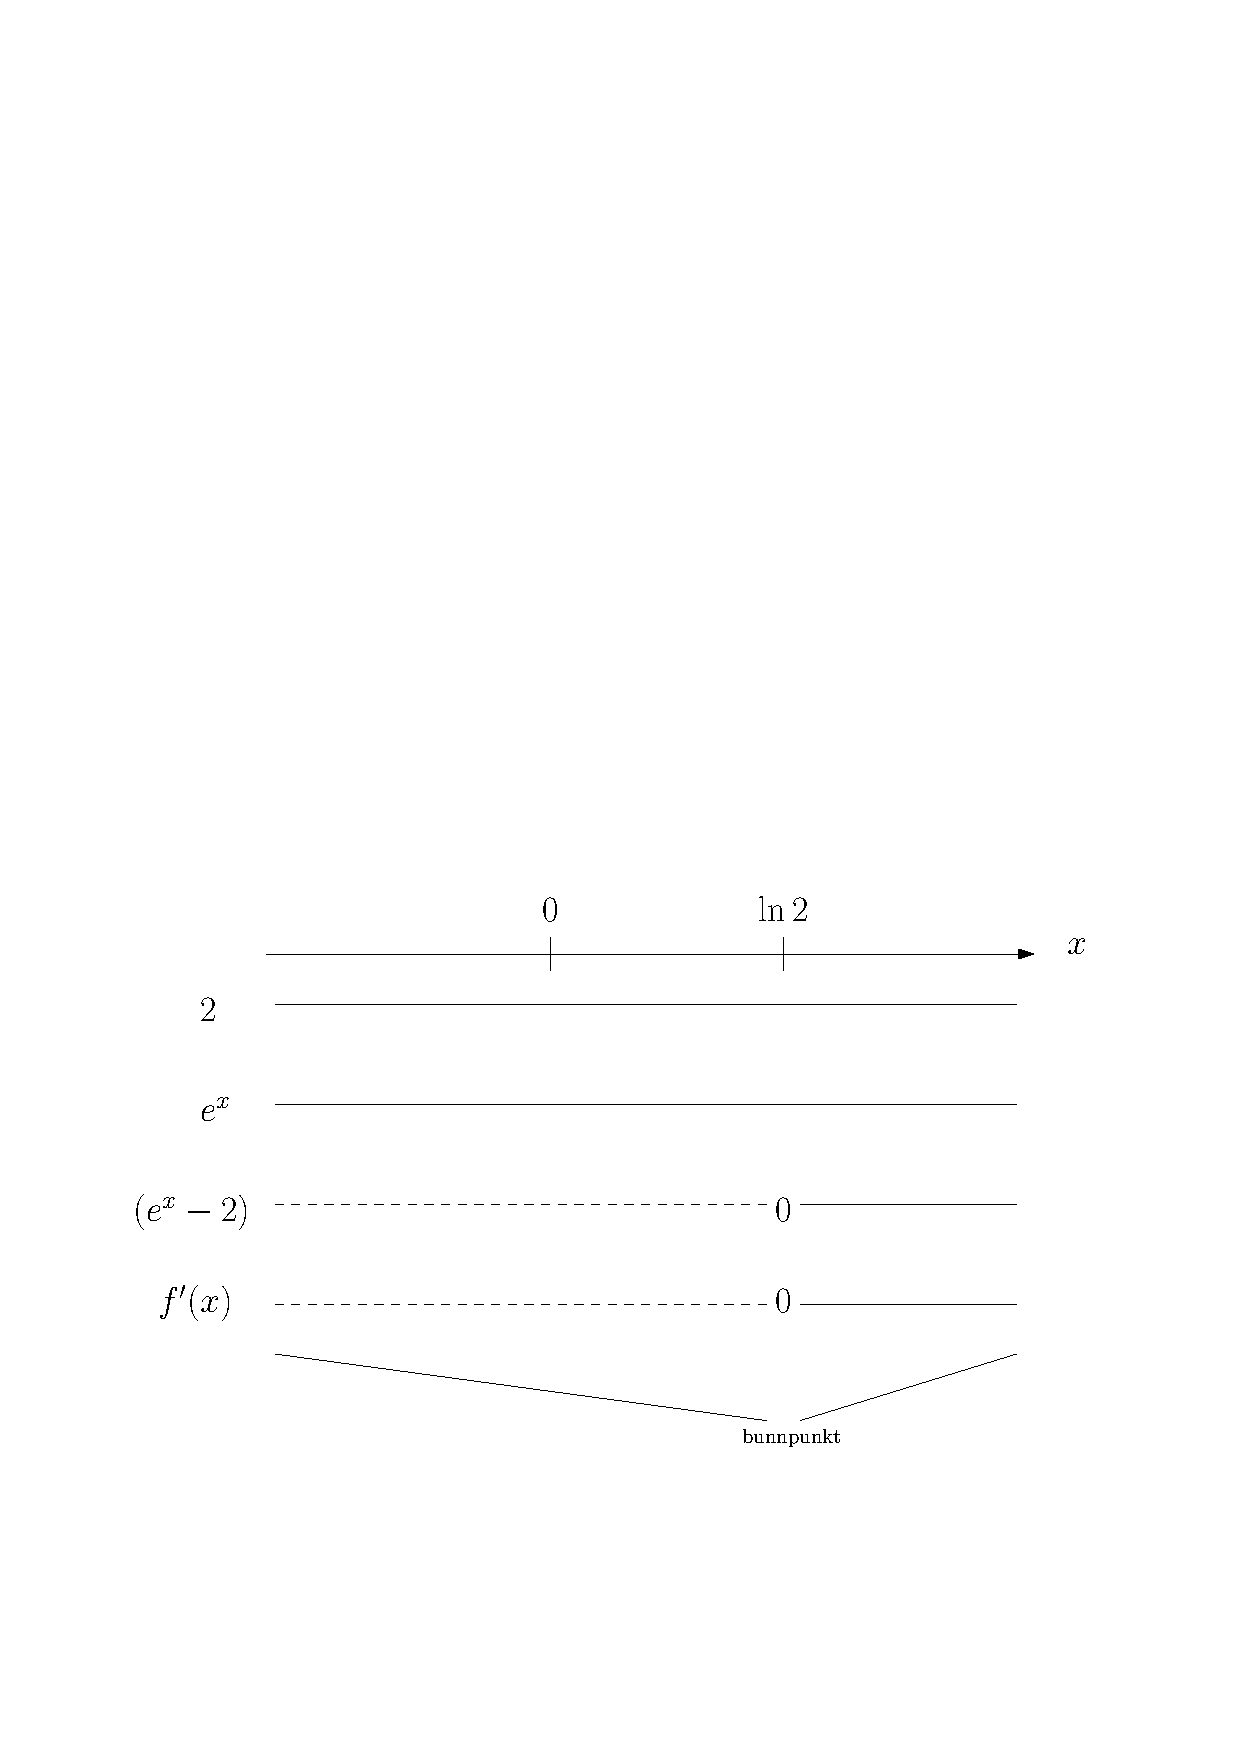
\includegraphics[width=0.75\linewidth]{figs/del1_oppg6b.pdf}
		\label{fig:del1_oppg6b}
	\end{figure}
	Vi ser av fortegnslinjen at vi har et bunnpunkt i $x = \ln 2$. Funksjonsverdien for denne $x$-verdien er
	\begin{equation*}
		f(\ln 2)  = e^{2\ln2} - 4e^{\ln 2} + 3 
		= e^{\ln 2^2} - 4e^{\ln 2} + 3  
		= 4 - 8 + 3 = -1
	\end{equation*}
	Bunnpunktet er altså $\answer{(\ln 2, -1)}$.
	
	
	# Når vi skal bestemme eventuelle vendepunkt, kan vi undersøke hvor den dobbeltderiverte av funksjonen endrer fortegn. 
	Vi deriverer derfor den deriverte vi fant i forrige deloppgave. 
	\begin{align*}
		f''(x) & = 4e^{2x} - 4e^x \\
		& = 4e^x(e^x -1)
	\end{align*}
	Deretter setter vi den dobbeltderiverte lik $0$, og lager igjen fortegnslinje som i oppgaven over.
	\begin{align*}
		f''(x) & = 0 \\
		4e^x(e^x-1) & = 0 \qquad \textnormal{$4e^x > 0$ alltid, så vi får}\\ 
		e^x -1 & = 0 \\
		x & = 0
	\end{align*}
	
	Fortegnslinjen vil se slik ut:
	\begin{figure}[ht!]
		\centering
		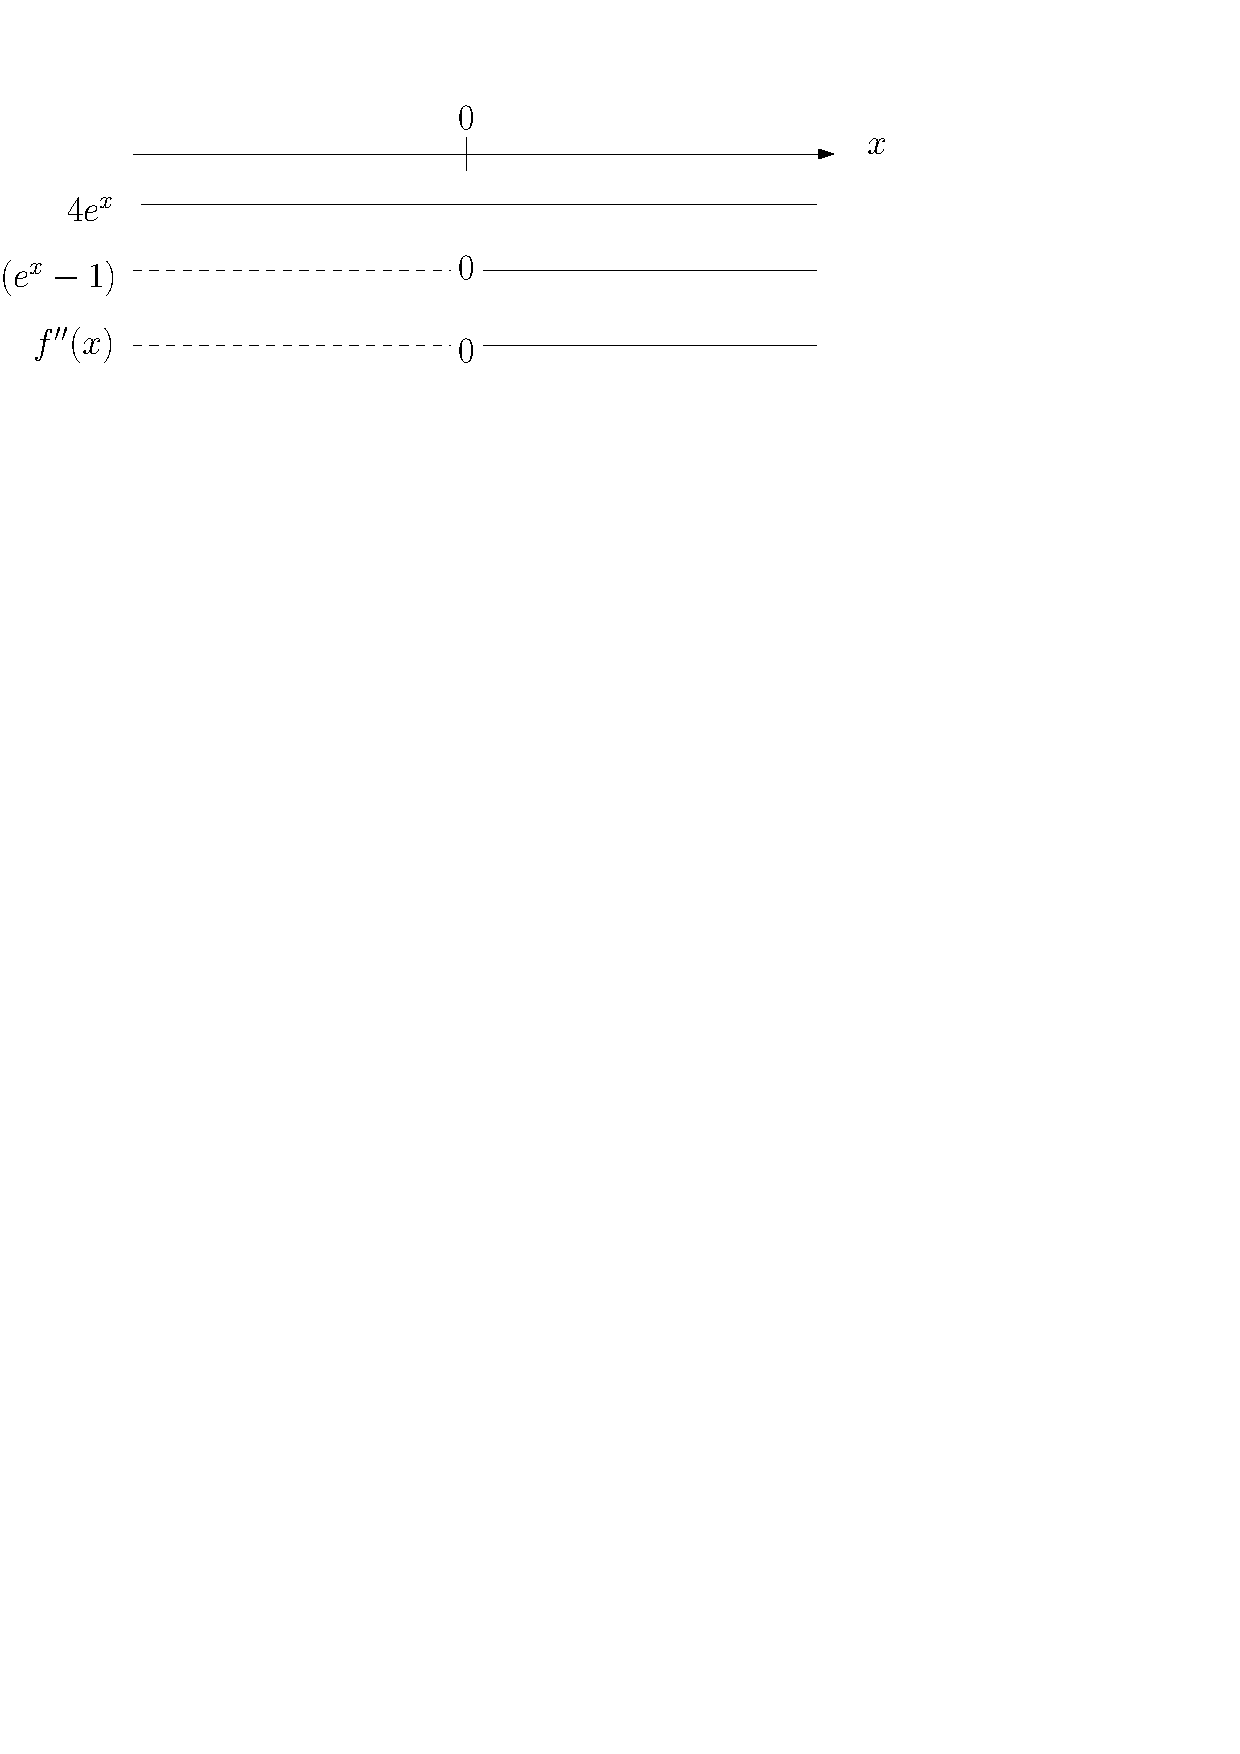
\includegraphics[width=0.75\linewidth]{figs/del1_oppg6c.pdf}
		\label{fig:del1_oppg6c}
	\end{figure}
	Vi ser altså at den dobbeltderiverte skifter fortegn når $x=0$. 
	Den tilhørende funksjonsverdien er: 
	\begin{equation*}
	f(0) = e^{2 \cdot 0} - 4e^0 + 3 = 1 -4 +3 = 0
	\end{equation*}	
	Vendepunktet for funksjonen er altså i punktet $\answer{(0,0)}$.
	
	# Når vi lager en skisse av grafen til funksjonen, er det veldig lurt å tegne inn de punktene vi har funnet i oppgavene over. 
	Disse punktene gir oss god informasjon om hvordan grafen omtrent kan se ut. 
	\begin{figure}[ht!]
		\centering
		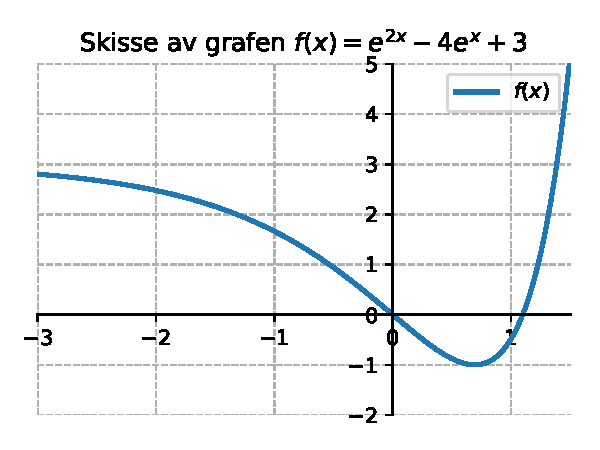
\includegraphics[width = 0.6\linewidth]{figs/del1_oppg6d.pdf}
		\label{fig:del1_oppg6d}
	\end{figure}
\end{easylist}


\subsection*{Oppgave 7}

\begin{easylist}[enumerate]
	\ListProperties(Style2*=,Numbers=a,Numbers1=l,FinalMark={)})
	
	# En måte å vise at trekantene er formlike på, er å sjekke at forholdet mellom samsvarende sider er det samme. 
	\begin{figure}[ht!]
		\centering
		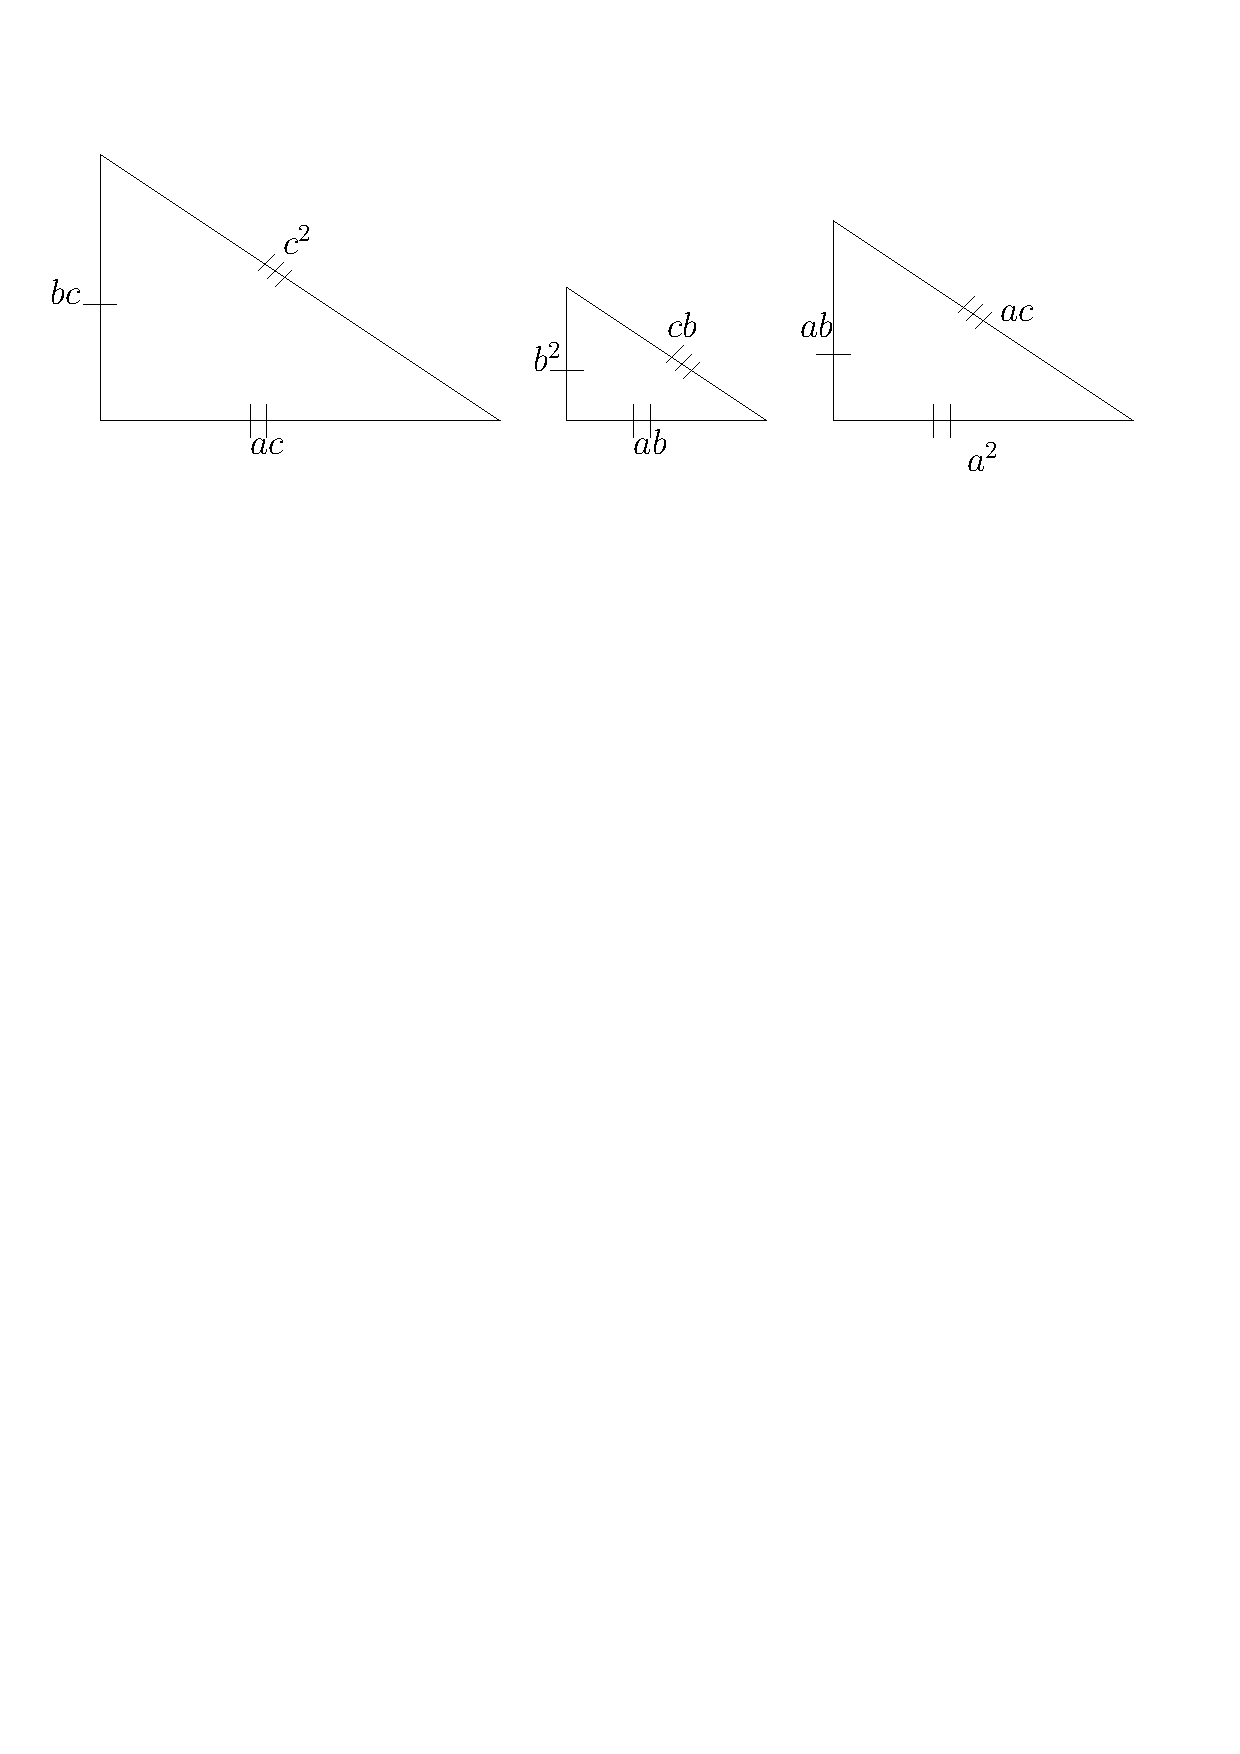
\includegraphics[width = 0.85\linewidth]{figs/del1_oppg7a.pdf}
		\label{fig:del1_oppg7a}
	\end{figure}	
	Vi starter med å vise at trekant 1 og 2 er formlike. Forholdet mellom de formlike sidene er:
	\begin{equation*}
			\frac{bc}{b^2}  = \frac{c}{b} \qquad \qquad
			\frac{ac}{ab}  = \frac{c}{b} \qquad \qquad
			\frac{c^2}{cb}  = \frac{c}{b}
	\end{equation*}
	Deretter sjekker vi om trekant 2 og 3 er formlike
	\begin{equation*}
			\frac{b^2}{ab} = \frac{b}{a} \qquad \qquad
			\frac{ab}{a^2} = \frac{b}{a} \qquad \qquad
			\frac{cb}{ac} = \frac{b}{a}
	\end{equation*}
	Vi ser altså at trekant 1 er formlik med trekant 2 og at trekant 2 er formlik med trekant 3. 
	Da må også trekant 1 og 3 være formlike. 
	
	# For å vise at punktene E, D og C ligger på en rett linje, må vi vise at $ \angle ADB + \angle ADE + \angle BDC = \ang{180} $. 
	Siden de tre trekantene er formlike, vet vi at samsvarende vinkler er like store. 
	Vi vet også at $\angle ADB = \ang{90}$, så det gjenstår å vise at $\angle ADE + \angle BDC = \ang{90}$.
	
	Dette gjør vi ved å trekke to hjelpelinjer som vist på figuren nedenfor. 
	Vi vet at to parallelle linjer som skjæres av samme linje danner samsvarende vinkler. 
	I tillegg får vi toppvinkler. Derfor vet vi at $\angle BAD$ er samsvarende vinkel med $\angle ADE$, som vil si at disse to vinklene er like store. 
	Vi får samme tilfelle for $\angle ABD$. 
	Denne er samsvarende med vinkel $\angle BDC$, altså er disse to vinklene også like store.
	\begin{figure}[ht!]
		\centering
		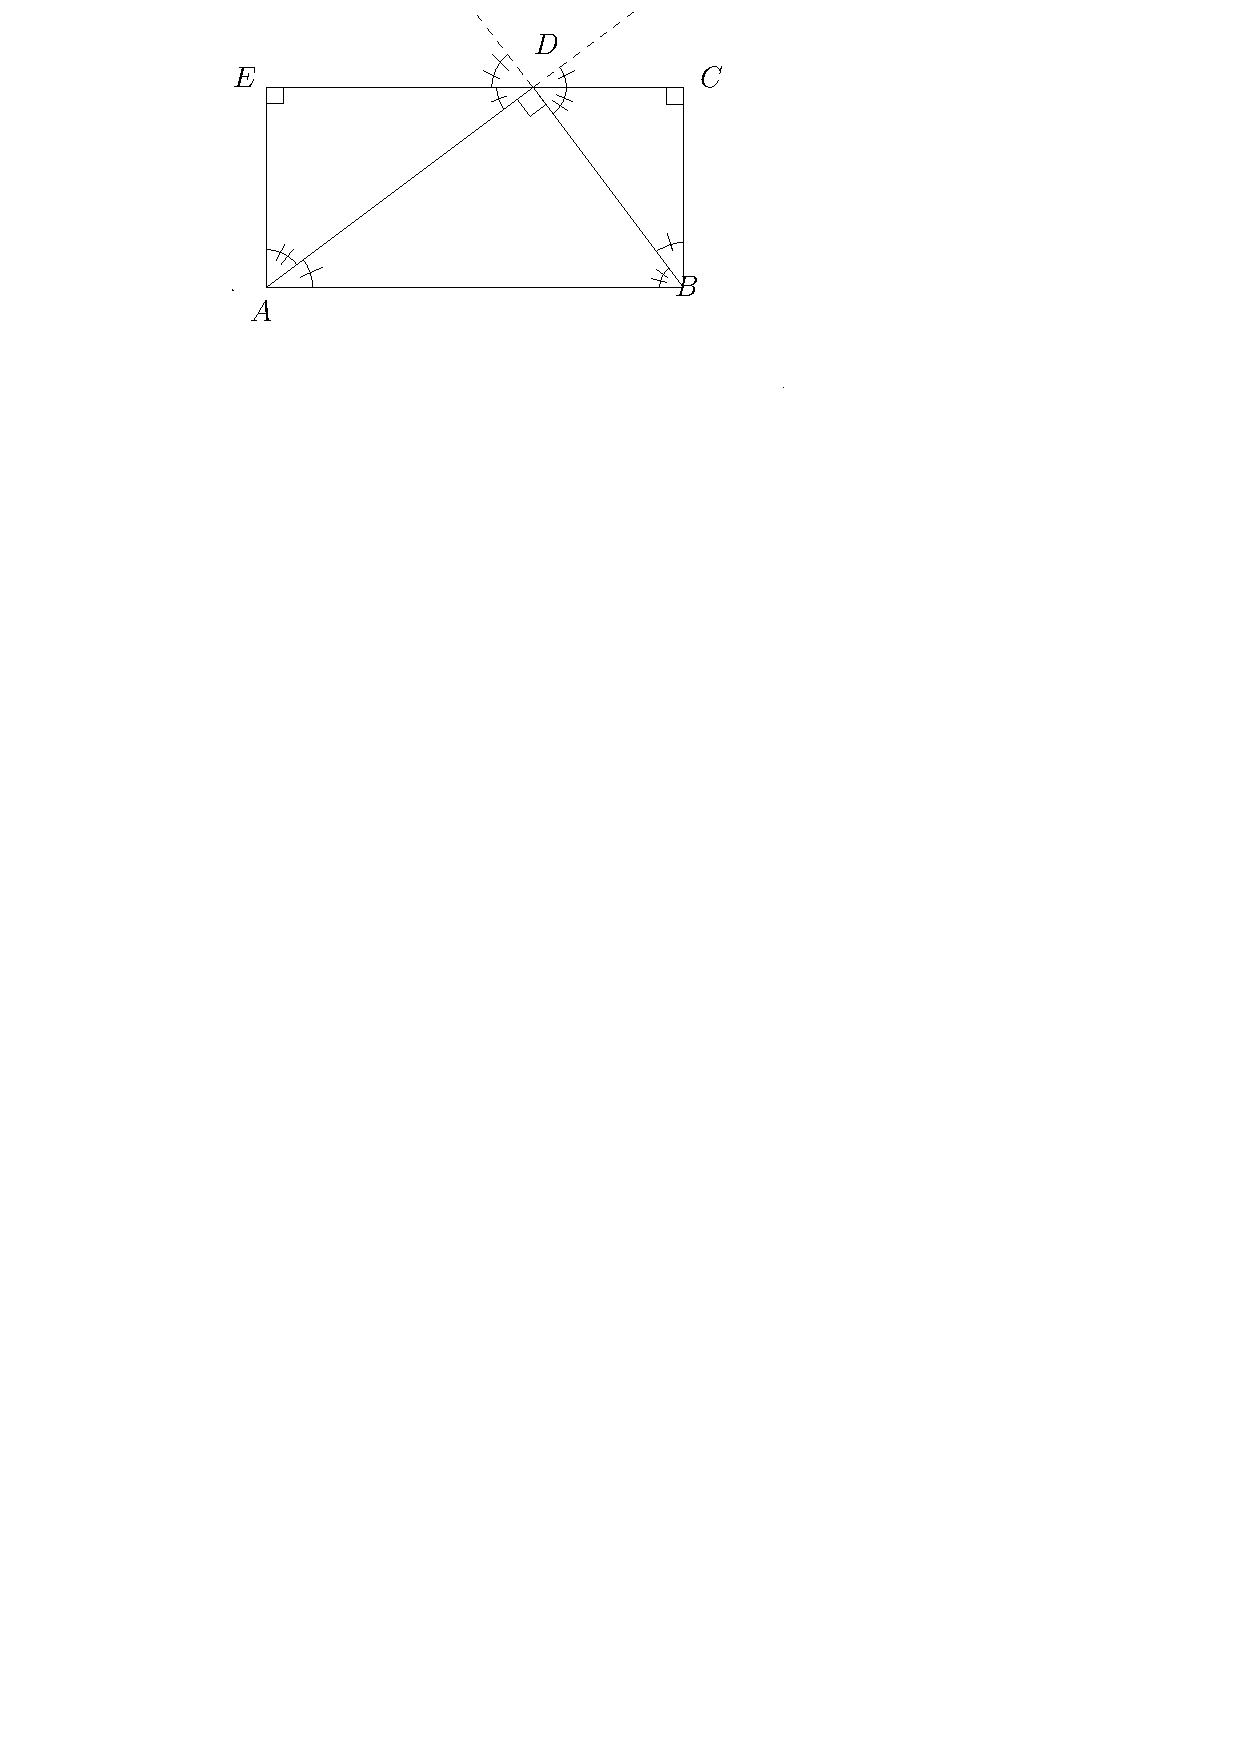
\includegraphics[width=0.7\linewidth]{figs/del1_oppg7b2.pdf}
		\label{fig:del1_oppg7b}
	\end{figure}
	Siden summen av vinklene i en trekant er $180$, vet vi at $\angle BAD + \angle  ABD = \ang{90}$, og dermed vet vi også at $\angle ADE + \angle BDC = \ang{90}$. 
	Vi har da at $\angle EDC  = \ang{180}$, og dermed må punktene E, D og C ligge på samme linje.
	
	# Fra oppgaven over har vi at $\angle DAE + \angle BAD = \ang{90}$ og at $\angle DBA + \angle CBD = \ang{90}$. 
	Da har vi at alle hjørnene i firkanten vår er $\ang{90}$, altså har vi et rektangel. 
	
	I et rektangel vet vi at parallelle sider er like lange, det vil si at lengden av siden EC skal være lik lengden av siden AB. 
	Altså: $a^2 + b^2 = c^2$, som er Pytagoras' setning.
\end{easylist}


\clearpage 
\section*{Del 2 - med hjelpemidler}

\subsection*{Oppgave 1}
\begin{easylist}[enumerate]
	\ListProperties(Style2*=,Numbers=a,Numbers1=l,FinalMark={)})
	
	# Først husker vi at vinkelen i en sirkel er $\ang{360}$. 
	Vi har en sentralvinkel i figuren, nemlig $u$. 
	Ettersom vinkelen i sirkelen må være $\ang{360}$ vet vi derfor at resten av vinkelen i sirkelen må være $\ang{360} - u$, siden da blir summen av de to vinklene lik $\ang{360}$. 
	Vinkel $\angle DCB$ spenner over buen $DB$, det samme gjør sentralvinkelen vi nettopp fant, $\ang{360} - u$. 
	Vi vet at periferivinkler som spenner over samme bue som en sentralvinkel vil være halvparten så stor som sentralvinkelen. 
	Dermed har vi 
	\begin{equation*}
		\angle DCB = \frac{1}{2} \cdot (\ang{360} - u) \\ = \ang{180} - \frac{1}{2}u
	\end{equation*}
	Altså har vi vist at $\answer{\angle DCB = \ang{180} - \frac{1}{2}u}$
	
	# Fra oppgave a) vet vi at $\angle DCB = \ang{180} - \frac{1}{2}u$. Vinkelen $\angle BAD$ er en periferivinkel som spenner over samme sirkelbue som sentralvinkelen $u$, derfor vet vi at  $\angle BAD = \frac{1}{2}u$. Legger vi nå sammen disse to vinkelene får vi:
	\begin{equation*}
		\angle BAD + \angle DCB = \ang{180} - \frac{1}{2}u + \frac{1}{2}u = \ang{180}
	\end{equation*}
	Videre er summen av vinkler i en firkant $\ang{360}$, derfor vet vi at $\angle CBA + \angle ADC = \ang{180}$.
	Dermed har vi vist at 
	\begin{equation*}
		\angle BAD + \angle DCB = \angle CBA + \angle ADC = \ang{180}.
	\end{equation*}
	
	
\end{easylist}
\subsection*{Oppgave 2}

\begin{easylist}[enumerate]
	\ListProperties(Style2*=,Numbers=a,Numbers1=l,FinalMark={)})

	Likningen for en sirkel kan skrives som
	\begin{equation*}
		x^2 + y^2 + ax + by + c = 0
	\end{equation*}
	og vi får oppgitt at $A(3,8)$, $B(9,6)$ og $C(13,-2)$ ligger på sirkelperiferien. 
	
	# For at likningen skal gjelde for en sirkel som går gjennom alle de gitte punktene, må likningen gå opp uansett hvilket punkt vi setter inn i likningen. 
	For å finne et likningssystem som svarer til det over, setter vi altså inn $x$- og $y$-koordinatene for hvert av punktene i hver sin likning. 
	Likningssystemet blir da:
	\begin{equation*}
		\begin{cases} 3^2 + 8^2 + 3a + 8b + c = 0
		\\ 9^2 + 6^2 + 9a + 6b + c = 0 
		\\ 13^2 + (-2)^2 + 13a - 2b + c = 0 
		\end{cases}
	\end{equation*}
	
	# Vi skriver inn hver likning i CAS, markerer alle linjene og trykker på \verb|x=|. 
	Vi kan også bruke kommandoen \verb|Løs|, og skrive inn hvilke linjer CAS skal løse. 
	Vi skriver inn \verb|Løs{$1, $2, $2}|, og får som svar at \answer{$a = -6, b = 4 \text{ og } c = -87$}.
	\begin{figure}[ht!]
		\centering
		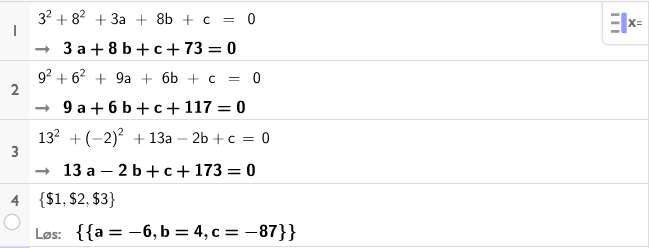
\includegraphics[width = 0.9\linewidth]{figs/del2_oppg2.png}
		\caption{Løsning på oppgave 2b) i CAS.}
		\label{fig:del1_oppg7}
	\end{figure}
\end{easylist}


\subsection*{Oppgave 3}
\begin{easylist}[enumerate]
	\ListProperties(Style2*=,Numbers=a,Numbers1=l,FinalMark={)})
	
	# For at vi i denne situasjonen skal kunne bruke en binomisk sannsynlighetsmodell må vi anta at alle delforsøkene er uavhengige. 
	Det vil i praksis si at dersom flere reiser sammen, så vil fremdeles alle i reisefølget møte opp eller ikke uavhengig av hva de andre i gruppen gjør.
	
	# Her kan vi bruke sannsynlighetskalkulatoren i GeoGebra. 
	Siden flyet har plass til maks 116 passasjerer, må vi undersøke hva sannsynligheten er for at 116 passasjerer eller mindre møter opp når selskapet har solgt 122 billetter. 
	I sannsynlighetskalkulatoren legger vi da inn $n = 122$, $p = 0.94$ og $P(X \leq 116)$. Resultatet blir da:
	\begin{figure}[ht!]
		\centering
		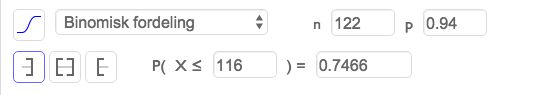
\includegraphics[width = 0.85 \linewidth]{figs/del2_oppg3b.png}
		\label{fig:del2_oppg3b}
	\end{figure}
	
	\answer{Sannsynligheten for at alle som møter får plass på flyet er 74.7 \%}

	# Siden vi skal finne ut hvor mange billetter selskapet kan selge, er det altså $n$ i denne oppgaven vi må bestemme. Da lar vi fremdeles $p = 0.94$, $P(X \leq 116)$, og så tester vi for hvilke verdier av $n$ som gjør at sannsynligheten vi får ut blir $\geq 95 \% $. Vi vet fra oppgaven over at de ikke kan selge 122 billetter, for da blir sannsynligheten for at alle får plass for liten i forhold til hva selskapet ønsker. Derfor kan vi prøve å sette inn for eksempel $n = 120$.
	\begin{figure}[ht!]
		\centering
		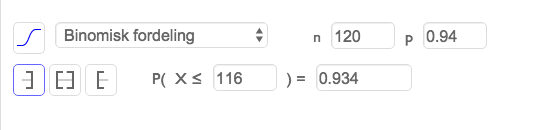
\includegraphics[width = 0.7 \linewidth]{figs/del2_oppg3c1.png}
	\end{figure}
	
	Vi ser at dette antallet også vil gi for liten prosent. Vi prøver da med for eksempel $n = 119$.
	
	\begin{figure}[ht!]
		\centering
		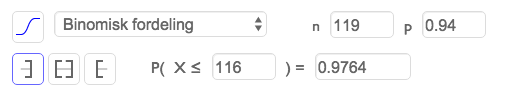
\includegraphics[width = 0.7 \linewidth]{figs/del2_oppg3c2.png}
	\end{figure}
	
	Dette ser vi gir en bedre prosent enn ønskelig, så flyselskapet kan altså selge \answer{119 billetter} og få at sannsynligheten er minst 95 \% for at alle som møter opp får plass på flyet.	
	
	
\end{easylist}

\subsection*{Oppgave 4}

\begin{easylist}[enumerate]
	\ListProperties(Style2*=,Numbers=a,Numbers1=l,FinalMark={)})
	
	# Her må vi først finne ut hvor lange sidene $s$ er som funksjon av $x$. 
	Da kan vi først se på trekant ABE. 
	Denne er likebeint, så vi vet at den rette linjen fra E ned til linjen AB vil danne $\ang{90}$ med linjen AB, og den vil dele AB i to like store deler. 
	Vi får altså to $\ang{90}$ trekanter, og da kan vi bruke Pytagoras' setning. 
	
	Den ene kateten vil da være halvparten av $AB$, altså $10/2$, mens den andre må vi lete litt mer etter.
	
	Vi ser at høyden i hele firkanten er 10, og at det er en lik trekant som ABE helt øverst i figuren også. 
	Det vil si at vi kan dele denne trekanten opp på samme måte som ABE og få en høyde også her. 
	Vi ser da av figuren at høydene i de to trekantene til sammen er $10-x$, og da vil høyden i hver av trekantene være $(10 - x)/ 2$. 
	Da har vi altså begge katetene og kan bruke Pytagoras' setning til å finne $s$.
	\begin{align*}
		s^2 &= \left (\frac{10-x}{2} \right)^2	+ \left(\frac{10}{2} \right)^2  
		= \sqrt{\left (\frac{10-x}{2} \right)^2 + \left(\frac{10}{2} \right)^2} \\
		 & = \sqrt{\frac{(10-x)^2}{4} + \frac{10^2}{4}}  
		 = \frac{1}{2} \sqrt{(10-x)^2 + 10^2} \\
		 & = \frac{1}{2} \sqrt{(x-10)^2 + 10^2} 		
	\end{align*}
	Den totale strekningen blir da
	\begin{equation*}
			g(x) = x + 4s = \answer{x + 2\sqrt{(x-10)^2 + 10^2}}.	
	\end{equation*}
	
	
	# Denne oppgaven kan gjøres på forskjellige måter i CAS. 
	Her velger vi å først skrive inn funksjonsuttrykket for $g(x)$, deretter derivere dette, og finne ut når den deriverte er $0$ ved å bruke kommandoen \verb|nullpunkt|. 
	Deretter sjekker vi hva den andrederiverte var i dette punktet. 
	Ettersom den andrederiverte var større enn $0$, vet vi at punktet vi fant er et bunnpunkt.
	
	
	\begin{figure}[ht!]
		\centering
		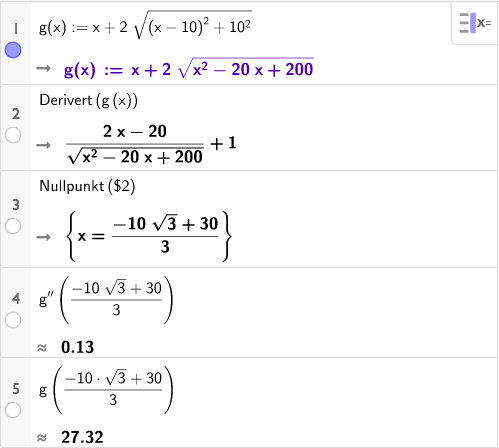
\includegraphics[clip, trim= 0cm 0cm 0cm 0cm, width = 0.70 \linewidth]{figs/del2_oppg4b.png}
	\end{figure}
	
	Den minste veilengden får vi altså når $x = \frac{-10 \sqrt{3} + 30}{3} \approx$ \answer{4.23 km}. Da er den totale veilengden \answer{27.32 km}.
\end{easylist}



\subsection*{Oppgave 5}

\begin{easylist}[enumerate]
	\ListProperties(Style2*=,Numbers=a,Numbers1=l,FinalMark={)})
	
	# Vi brukerkommandoen \\
	\verb|Kurve(Uttrykk, Utrykk, Parametervariabel, Start, Slutt)|.
	\begin{figure}[ht!]
		\centering
		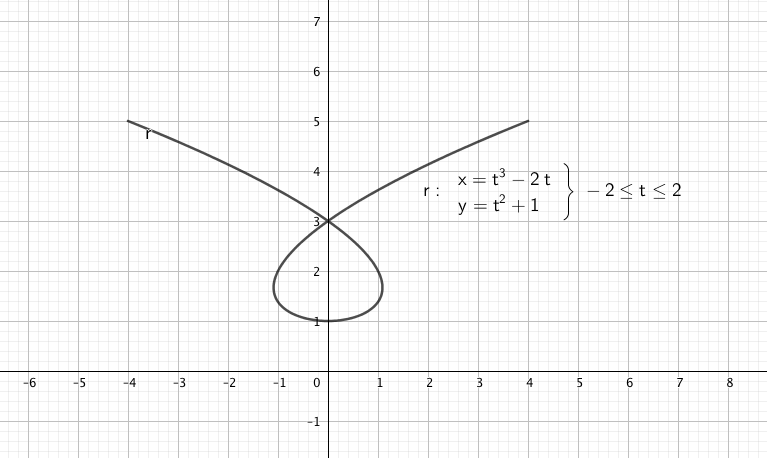
\includegraphics[width = 0.85\linewidth]{figs/del2_oppg5a.png}
	\end{figure}
	
	# Fartsvektoren er den deriverte av posisjonsvektoren.
	\begin{align*}
			\vec{v}(t) & = \vec{r} \, '(t)  = [3t^2 -2, 2t] \\
			\vec{v}(-1) & = [3(-1)^2,2(-1)] \\
			& = [3-2,-2] = [1,-2] 
	\end{align*}
	Videre har vi at banefarten er 
	\begin{equation*}
		|\vec{v}(t)| = \sqrt{1^2 + (-2)^2} = \sqrt{1 + 4} = \sqrt{5}
	\end{equation*}
	For å tegne inn denne vektoren i graftegneren bruker vi kommandoen \\ \verb|Vektor(startpunkt, sluttpunkt)|. 
	Vi vet at startpunktet skal være i $\vec{r}(-1)$, og at sluttpunktet vil være der $\vec{v}(-1)$ slutter.
	Vektoren går altså fra punktet $\vec{r}(-1)$ til punktet $\vec{r}(-1) + \vec{r}\, '(-1)$.

	\begin{figure}[ht!]
		\centering
		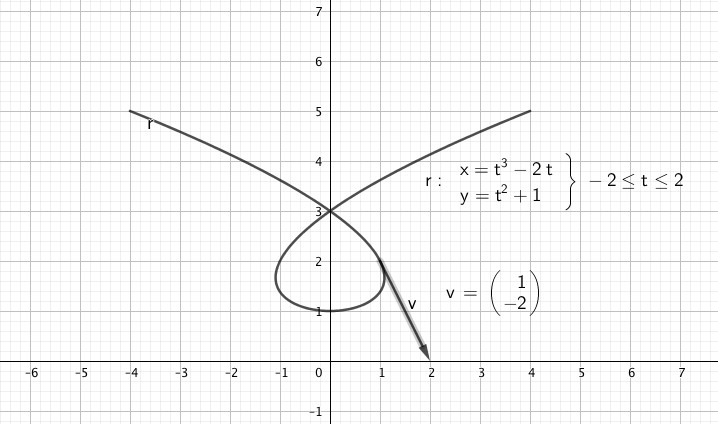
\includegraphics[clip, trim= 0cm 0cm 0cm 3cm, width = 0.85\linewidth]{figs/del2_oppg5b.png}
	\end{figure}
	
	# Dette kan gjøres på flere måter. 
	Her velger vi å først definere formelen for banefarten. 
	Deretter løser vi $v = 2$. 
		\begin{figure}[ht!]
			\centering
			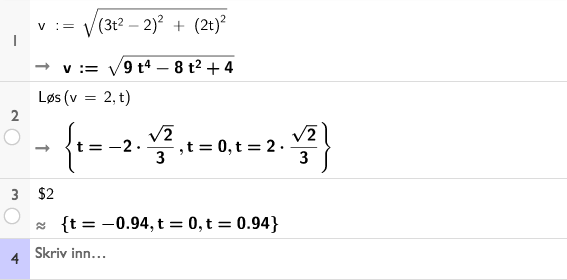
\includegraphics[width = 0.85\linewidth]{figs/del2_oppg5c.png}
		\end{figure}
		
	Banefarten er altså 2 når \answer{$t = -0.94$, $t=0$ og når $t = 0.94$}.
		
	# Denne oppgaven kan også fint løses i CAS med samme tankegang som brukes under. 
	Først finner vi akselerasjonsvektoren. 
	Dette er den deriverte av fartsvektoren. 
	Deretter sjekker vi hvilke $t$-verdier som gjør at skalarproduktet mellom de to vektorene er $0$. 
	Dette gjør vi fordi vi vet at hvis skalarproduktet mellom to vektorer er 0, må vinkelen mellom dem være $\ang{90}$.
	Vi har at $\vec{a}(t)  = \vec{v} \, '(t)  = [6t,2]$, og at
	\begin{align*}
			\vec{a}(t) \cdot \vec{v}(t) &= 0 \\
			[3t^2 -2,2t] \cdot [6t,2] & = 0 \\
			(3t^2 - 2) \cdot 6t + 2t \cdot 2  & = 0\\
			18t^3 - 12t + 4t & = 0 \\
			18t^3 - 8t & = 0 \\
			2t(9t^2 -4) & = 0 
	\end{align*}
	Da får vi enten $t = 0$, eller $9t^2 = 0$. 
	Vi må løse siste likning også for $t$.
	\begin{equation*}
			9t^2 -4  = 0 \qquad
			t^2  = \frac{4}{9} \qquad
			t = \pm \frac{2}{3}
	\end{equation*}
		
	De to vektorene står altså vinkelrett på hverandre når $t = 0$ og når $t = \pm 2/3$.
		
	Deretter sjekker vi når banefarten får sine ekstremalpunkter. Dette gjør vi ved å derivere banefarten og se når denne er lik 0.
		\begin{align*}
	|\vec{v}(t)| & = \sqrt{(3t^2 - 2)^2 + (2t)^2} 
	= \sqrt{9t^4 - 12t + 4 +4t^2} \\
				 & = \sqrt{9t^4 - 8t^2 + 4} = (9t^4 - 8t^2 + 4)^{\frac{1}{2}} \\
|\vec{v}(t)| '   &= \frac{1}{2} \cdot (9t^4 - 8t^2 + 4)^{-\frac{1}{2}} \cdot (36t^3 -16t) \\
				 & = \frac{18t^3 - 8t}{\sqrt{9t^4 - 8t^2 + 4}} 
		\end{align*}
		Den deriverte er 0 når telleren er 0.
		\begin{align*}
				18t^3 - 8t & = 0 \\
				2t(9t^2 -4) & = 0 
		\end{align*}
		Dette ser vi er akkurat samme likning som vi hadde lengre oppe. 
		Dermed vil løsningene være de samme. 
		Vi har vist at banefarten har sine ekstremalpunkter i de punktene der fartsvektoren står normalt på akselerasjonsvektoren.
		
\end{easylist}
\textbf{Kommentar.}
Hvorfor er det egentlig slik?
Dersom $v(t) = [v_x(t), v_y(t)]$, så har banefarten $|v(t)| = \sqrt{v_x^2(t) +  v_y^2(t)}$ ekstremalverdi når den deriverte er lik null.
Fordi $f(t) = \sqrt{g(x)}$ har derivert $f'(t) = g'(t) / (2 \sqrt{g(x)})$ ved bruk av kjernereglen, er $|v ' (t)| = 0$ når $2v_x(t) v_x'(t) +  2v_y(t) v_y'(t) = 0$. Her har vi også brukt kjerneregelen til å derivere $v_x^2(t)$.
Dette er akuratt samme likning som 
\begin{equation*}
	v(t) \perp a(t) = v(t) \perp v \, '(t) = v_x(t) v_x ' (t) + v_y(t) v_y ' (t) = 0,
\end{equation*}
og derfor er påstanden i deloppgave d) alltid sann.







\end{document}